%----------------------------------------------------------------------------
\appendix
%----------------------------------------------------------------------------
\chapter*{\fuggelek}\addcontentsline{toc}{chapter}{\fuggelek}
\setcounter{chapter}{\appendixnumber}
%\setcounter{equation}{0} % a fofejezet-szamlalo az angol ABC 6. betuje (F) lesz
\numberwithin{equation}{section}
\numberwithin{figure}{section}
\numberwithin{lstlisting}{section}
%\numberwithin{tabular}{section}

%----------------------------------------------------------------------------
\section{Állapottérképek elemei}
%----------------------------------------------------------------------------
%\begin{figure}[!ht]
%\centering
%\includegraphics[width=150mm, keepaspectratio]{figures/TeXstudio.png}
%\caption{A TeXstudio \LaTeX-szerkesztő.} 
%\end{figure}

\begin{figure}[!ht]
	\centering
	
\includegraphics[keepaspectratio]{figures/statechart_elements/states.png}
	\caption{Állapotok és köztük definiált állapotátmenet, triggerrel, őrfeltétellel és actionnel}
\end{figure}

\begin{figure}[!ht]
	\centering
	
\includegraphics[keepaspectratio, width=80mm]{figures/pseudo-and-final.png}
	\caption{Kezdőállapot, DeepHistory, ShallowHistory, Termináló állapot és Végállapot}
\end{figure}

\begin{figure}[!ht]
	\centering
	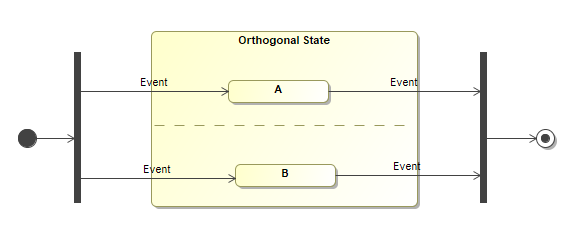
\includegraphics[keepaspectratio, width=100mm]{figures/statechart_elements/forkjoin.png}
	\caption{Példa: fork-join}
\end{figure}

\begin{figure}[!ht]
	\centering
	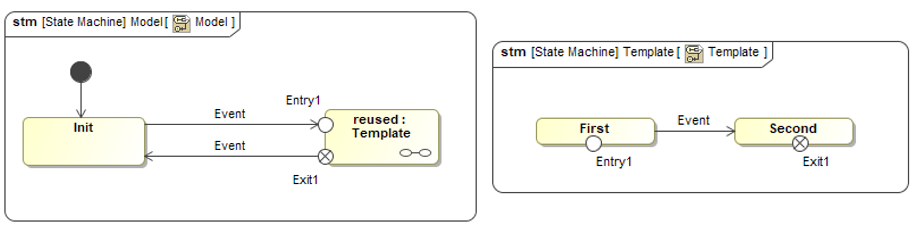
\includegraphics[keepaspectratio, width=150mm]{figures/statechart_elements/SubmachineState.png}
	\caption{Állapottérkép újrafelhasználása Submachine State segítségével}
\end{figure}

\begin{figure}[!ht]
	\centering
	\fbox{
\includegraphics[keepaspectratio, width=70mm]{figures/choice.png}}\vspace{1cm}	
	\fbox{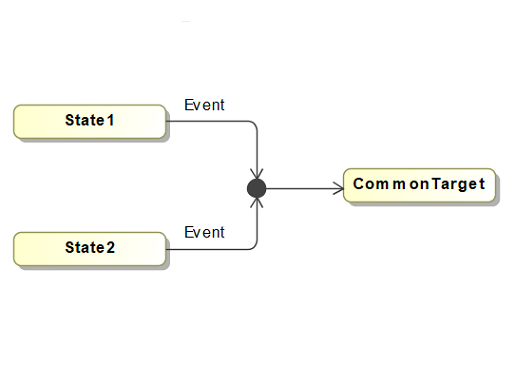
\includegraphics[keepaspectratio, width=70mm]{figures/junction.png}}
	\caption{Döntés és Csomópont szintakitkája}
\end{figure}

\clearpage\section{Gamma Statechart Language}

\begin{figure}[!ht]
	\begin{lstlisting}
	package Exapmle
	
	statechart MonitorStatechart [] {
	
	transition from Red to Blue
	transition from Entry0 to Red
	
	region main_region {
	initial Entry0
	state Red
	state Blue
	}
	}
	\end{lstlisting}
	\caption{Gamma Statechart konkrét szöveges szintaxisa}
\end{figure}


\begin{figure}[!ht]
	\centering
	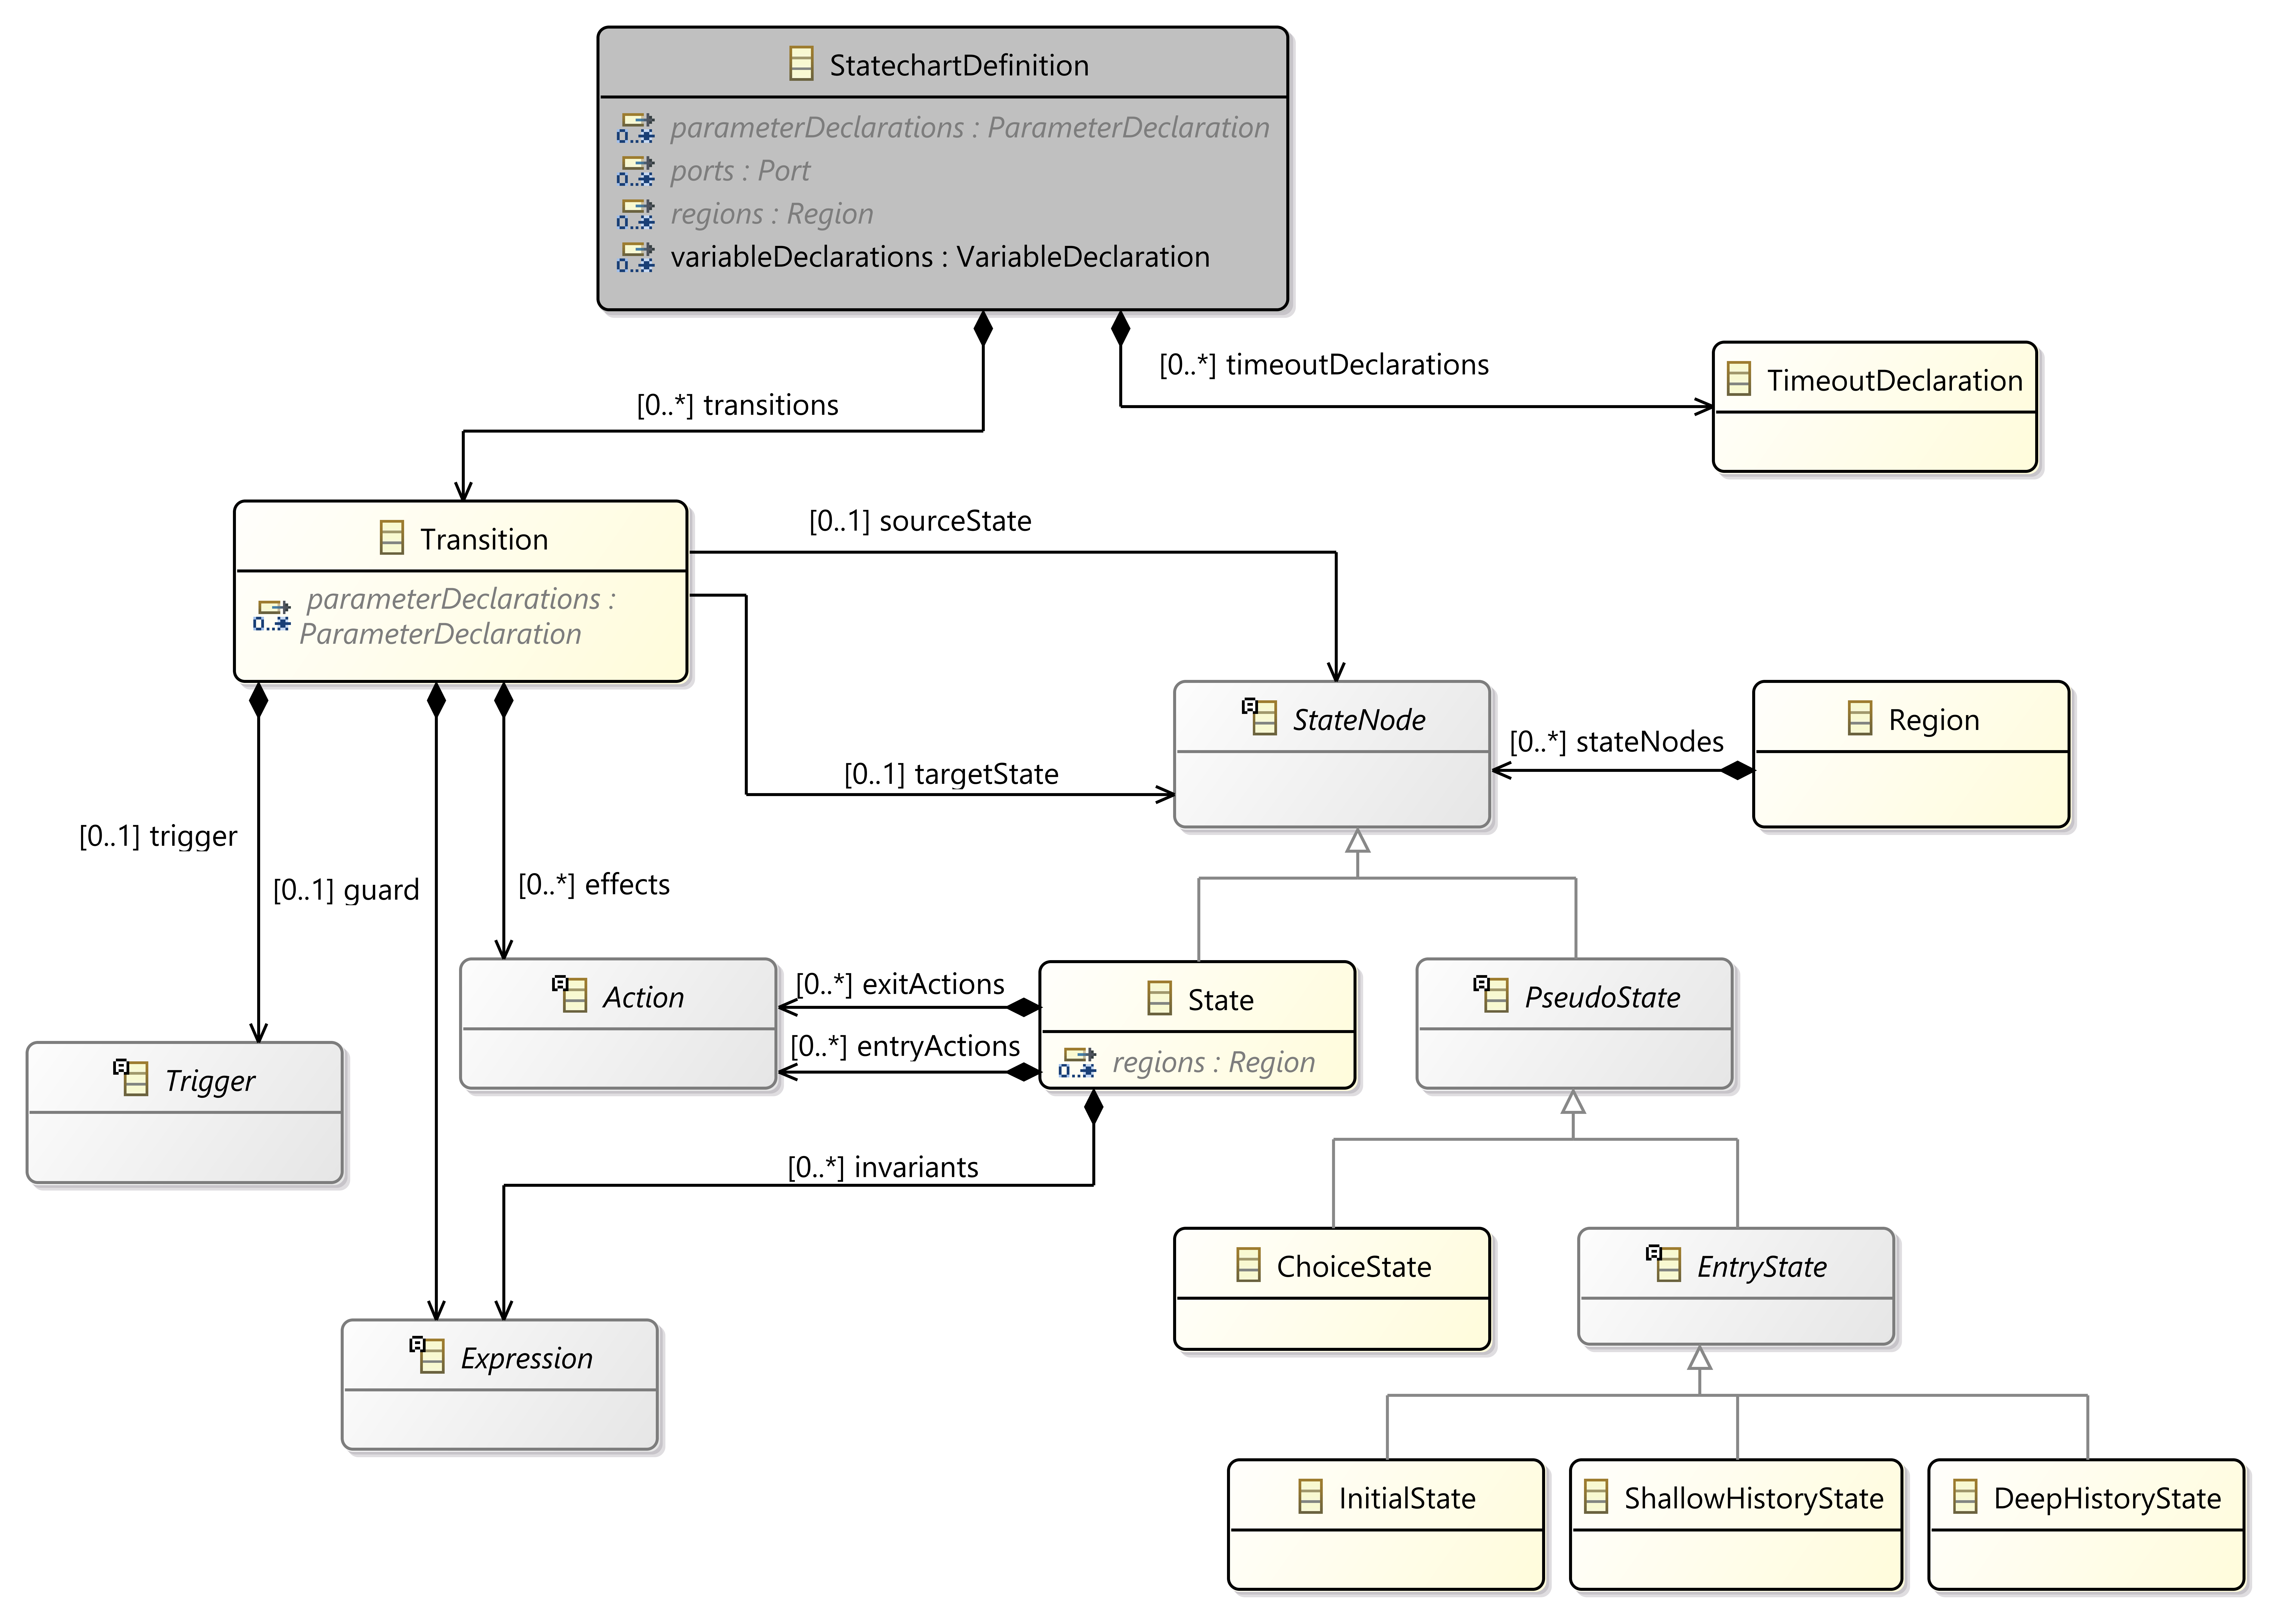
\includegraphics[keepaspectratio, width=150mm]{figures/statechart_class_diagram.png}
	\caption{Gamma állapottérkép absztrakt szintaxisa}
\end{figure}

\clearpage\section{Koncepció}

\begin{figure}[!ht]
	\centering
	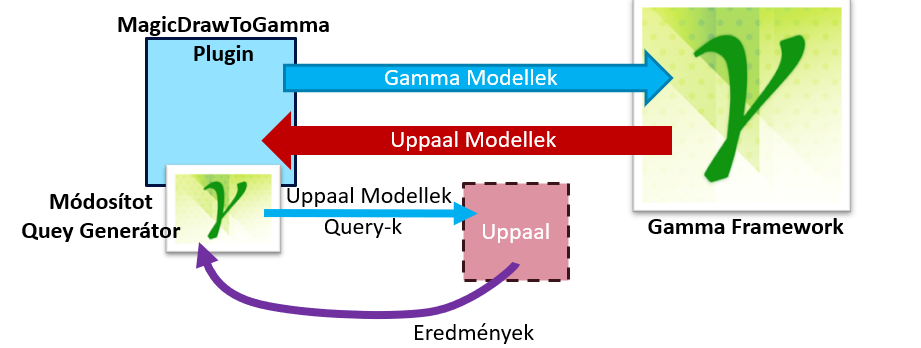
\includegraphics[keepaspectratio, width=150mm]{figures/concept.png}
	\caption{Koncepció}
\end{figure}

\section{Esettanulmány}

\begin{figure}[H]
	\centering
	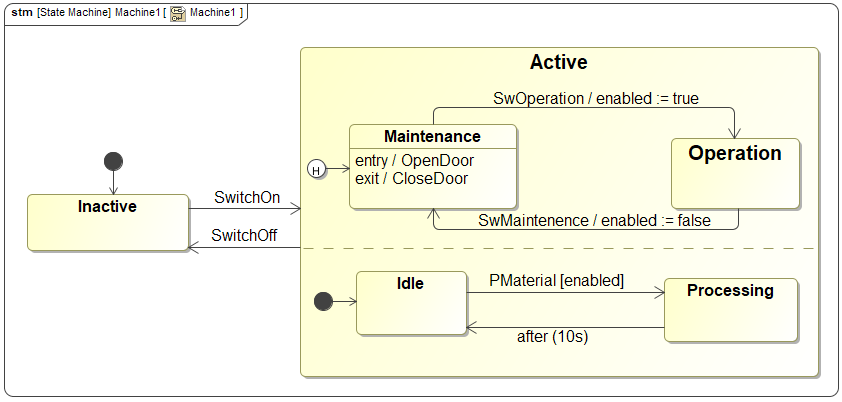
\includegraphics[keepaspectratio, width=150mm]{figures/machine1.png}
	\caption{Lehetséges leírás}
\end{figure}

\begin{figure}[H]
	\centering
	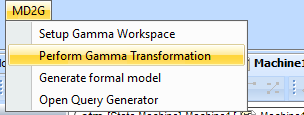
\includegraphics[keepaspectratio, width=70mm]{figures/GammaTrafo.png}
	\caption{MD2G menüpontok}
\end{figure}

\begin{figure}[H]
	\centering
	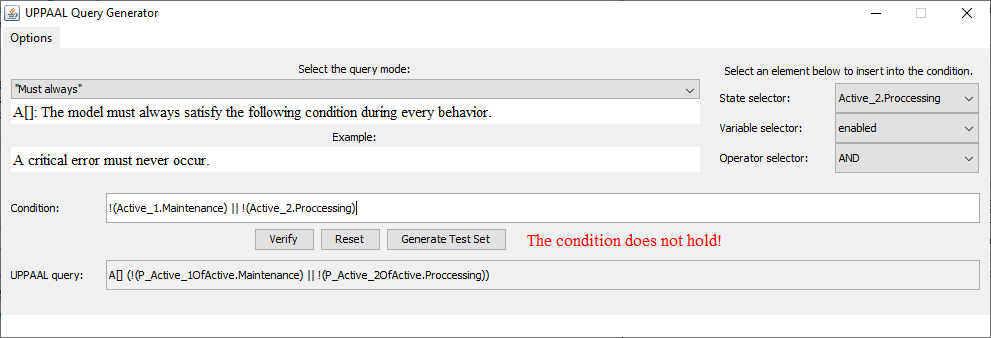
\includegraphics[keepaspectratio, width=150mm]{figures/query-gen-result.png}
	\caption{Verifikáció eredménye}
\end{figure}

\begin{figure}[H]
	\centering
	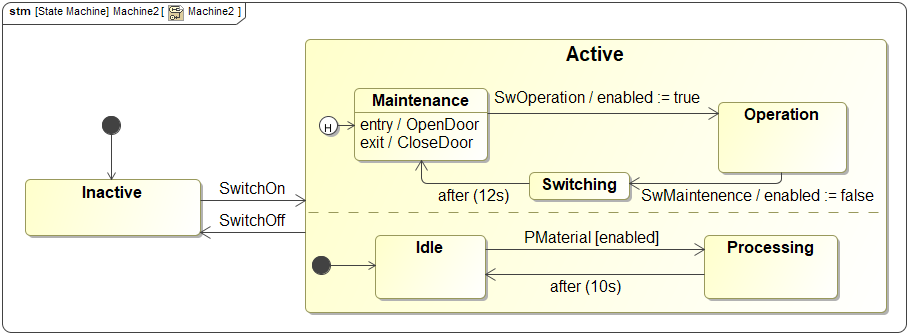
\includegraphics[keepaspectratio, width=150mm]{figures/machine2.png}
	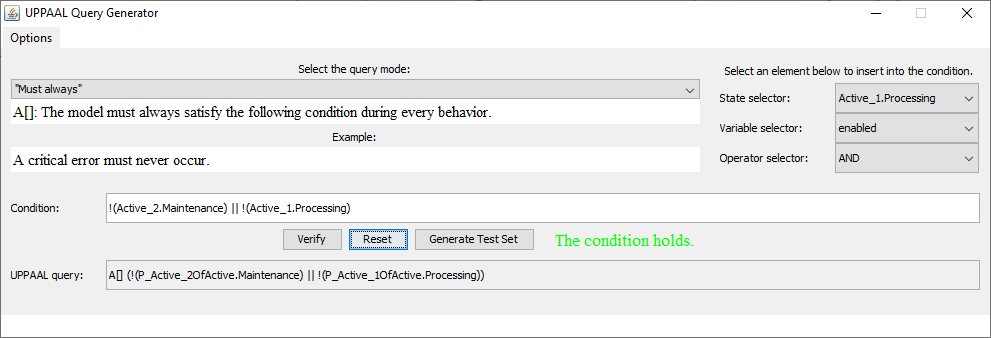
\includegraphics[keepaspectratio, width=150mm]{figures/fixed-result.png}
	\caption{Módosított állapottérkép és a verifikáció eredménye}
\end{figure}

\clearpage\section{Mérések}

\begin{figure}[H]
	\centering
	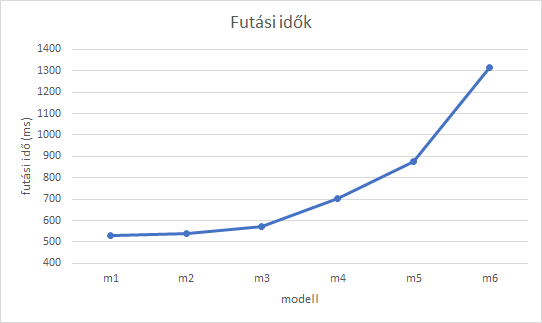
\includegraphics[keepaspectratio, width=140mm]{figures/meres1.png}
	\caption{Első mérés: transzformációk egymás után növekvő modellen}
\end{figure}

\begin{figure}[H]
	\centering
	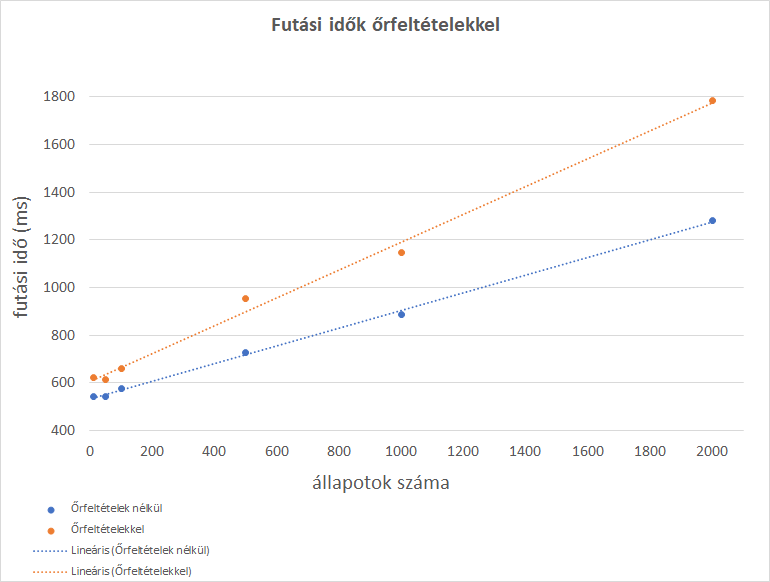
\includegraphics[keepaspectratio, width=140mm]{figures/meres2.png}
	\caption{Második mérés: futási idők őrfeltételekkel}
\end{figure}

\clearpage \section{Kódrészletek}
\begin{figure}[!ht]
	\lstset{style=javacode}
	\begin{lstlisting}
public class MyPlugin extends com.nomagic.magicdraw.plugins.Plugin {
	public void init(){
	//plugin belépési pontja
	}
	
	public boolean close(){
	//plugin leáll
	}
	
	public boolean isSupported(){
	//feltételek teljesülése a plug-in betöltéséhez
	return true;
	}
}
	\end{lstlisting}
	\caption{MagicDraw plugin osztály kódja}
\end{figure}

\begin{figure}[!ht]
	\lstset{style=VQL}
	\begin{lstlisting}
pattern RegionsInRegion(container: Region, region: Region){
	Region.subvertex(container, vertex);
	State.region(vertex, region);
}
	pattern RegionsInStatemachine(stateMachine: StateMachine, subregion: Region){
	find MainRegions(stateMachine, subregion);
} or {
	find RegionsInRegion+(region, subregion);
	StateMachine.region(stateMachine, region);
}
pattern TranisitonsInStateMachine(stateMachine: StateMachine, transition: Transition){
	find RegionsInStatemachine(stateMachine, region);
	Region.transition(region, transition);
}
	\end{lstlisting}
	\caption{állapotátmenetek megkeresése VQL-el}
\end{figure}
\begin{figure}[!ht]
\lstset{style=javacode}
\begin{lstlisting}
Injector injector = new StatechartLanguageStandaloneSetup()
	.createInjectorAndDoEMFRegistration();

ParserRule rule = injector.getInstance(StatechartLanguageGrammarAccess.class)
	.getExpressionRule();

IParseResult result = injector.getInstance(StatechartLanguageParser.class)
	.parse(rule, new StringReader(guardString));
\end{lstlisting}
\caption{Parse-olás Xtextel}
\end{figure}

\begin{figure}[!ht]
\lstset{style=VQL}
\begin{lstlisting}
pattern DeclarationsByName(statechartDefinition: StatechartDefinition, name: java String, declaration: Declaration){
	StatechartDefinition.variableDeclarations(statechartDefinition, declaration);
	Declaration.name(declaration, name);
}
\end{lstlisting}
\caption{Változók deklarációjának név szerinti megkeresése}
\end{figure}




